
\documentclass{jtetiproposalskripsi}

%-----------------------------------------------------------------
%Disini awal masukan untuk data proposal skripsi
%-----------------------------------------------------------------
\titleind{Sistem Informasi Nilai Berbasis SMS Gateway Program Diploma Universitas Muhammadiyah Jember.}
\fullname{SHIBGOHTULLAH AZZAM A.M.}

\idnum{1200631024}

\approvaldate{07 Februari 2015}

\degree{Sarjana Teknik Elektro}

\yearsubmit{2015}

\program{Manajemen Informatika}

\headprogram{Bagus Setya Rintyarna, S.T, M. Kom}

\firstsupervisor{Triawan Adi Cahyanto, M. Kom}
\firstnip{12 03 719}

\secondsupervisor{Bagus Setya Rintyarna, S.T, M. Kom}
\secondnip{09 03 521}


%-----------------------------------------------------------------
%Disini akhir masukan untuk data proposal skripsi
%-----------------------------------------------------------------

\begin{document}

\cover

\approvalpage

%-----------------------------------------------------------------
%Disini akhir masukan untuk muka skripsi
%-----------------------------------------------------------------

%-----------------------------------------------------------------
%Disini awal masukan Intisari
%-----------------------------------------------------------------
\begin{abstractind}
Teknologi informasi yang berkembang pesat dewasa ini, telah mendorong percepatan di berbagai bidang. Hal ini juga yang menyebabkan munculnya kemajuan pada perangkat lunak dan diimbangi pula dengan kemajuan dan kecanggihan teknologi beserta perangkat kerasnya. Secara langsung ataupun tidak, teknologi informasi telah menjadi bagian penting dari berbagai bidang kehidupan. Karena banyak kemudahan yang ditawarkan, teknologi informasi hampir tidak dapat dilepaskan dari berbagai aspek kehidupan manusia.
\paragraph{}
Salah satu teknologi informasi yang sangat populer saat ini adalah handphone beserta fasilitas SMS (Short message Service). Handphone sudah menjadi semacam identitas diri secara personal. Karena sifatnya yang personal maka, semua info yang masuk ke dalam handphone dirasakan oleh penggunanya sebagai bentuk informasi personal. Ditambah lagi dari secara psikologi bahwa seseorang itu ingin selalu  dianggap penting. Jadi apapun jenis SMS yang masuk, orang tersebut pasti akan membuka dan membacanya. 
\paragraph{}
Polling merupakan salah satu alat bantu yang bagus dalam mengambil keputusan. Dengan polling, kita bisa mengetahui pendapat banyak orang mengenai  permasalahan tertentu tanpa debat berkepanjangan, dalam hal ini penulis mencoba  memanfaatkan teknologi SMS sebagai media penyampaian suara dalam pengambilan  keputusan. Selanjutnya penulis akan menampilkan hasil polling dalam bentuk website, sehingga dapat diakses secara global. 
\paragraph{}
Oleh sebab itu penulis mencoba merancang sebuah sistem polling dengan SMS Gateway. Dengan adanya polling SMS ini diharapkan kita dapat melakukan polling dengan cepat dan memperoleh informasi hasil polling dengan mudah dan akurat.

\end{abstractind}
%-----------------------------------------------------------------
%Disini akhir masukan Intisari
%-----------------------------------------------------------------

\tableofcontents
\addcontentsline{toc}{chapter}{DAFTAR ISI}
\selectlanguage{bahasa}\clearpage\pagenumbering{arabic}\setcounter{page}{1}

%-----------------------------------------------------------------
%Disini awal masukan untuk Bab
%-----------------------------------------------------------------
\chapter{LATAR BELAKANG}

\section{Latar Belakang Masalah}
Teknologi informasi merupakan teknologi yang menggabungkan antara komputasi dan komunikasi untuk melakukan tugas-tugas informasi sehingga arus informasi dapat berjalan dengan baik. Teknologi Informasi berkembang dengan pesat di berbagai aspek kehidupan, mulai dari personal hingga instansi. Dalam sebuah instansi baik negeri maupun swasta, teknologi informasi sangat dibutuhkan untuk optimalisasi segala proses yang berkaitan dengan pembangunan dan perbaikan sistem. Salah satu bentuk optimalisasi tersebut adalah penerapan sistem informasi. Kriteria dari sistem informasi antara lain adalah fleksibel, efektif dan efisien. 
\paragraph{}
Dengan menggunakan perkembangan teknologi yang pesat, proses penyampaian informasi saat ini menjadi lebih mudah. Sarana penyampaian informasi yang paling populer dan mudah didapatkan saat ini adalah melalui handphone / ponsel. Layanan SMS(Short message Service) yang dimiliki setiap ponsel dapat kita gunakan untuk melayani informasi – informasi yang dibutuhkan, dalam hal ini informasi nilai program Diploma Universitas Muhammadiyah Jember kepada mahasiswa. 
\paragraph{}
Saat ini proses penyampaian informasi yang dimiliki oleh instansi Program Pasca Sarjana masih dilakukan secara manual atau mahasiswa harus datang langsung ke Universitas sehingga menjadi boros waktu dan biaya. Selain boros, mahasiswa juga sulit untuk mendapatkan informasi update nilai yang terbaru terutama yang lokasi tempat tinggal mahasiswa jauh dari Universitas. Bertitik tolak dari keinginan di atas maka kami mengusulkan program ini dengan harapan semoga ke depan sistem informasi nilai yang dimiliki universitas ini akan lebih baik.



\section{Rumusan Masalah}
Berdasarkan uraian tersebut maka dapat dirumuskan bagaimana membuat Sistem informasi nilai berbasis \textit{SMS Gateway} Program Diploma Universitas Muhammadiyah Jember.

\section{Batasan Masalah}
Untuk menghindari melebarnya masalah maka penulis membatasi masalah hanya pada proses pemberian informasi nilai atau IP (Index Prestasi) kepada mahasiswa berbasis \textit{SMS Gateway}. Sedangkan data nilai / IP tersebut dimasukkan oleh seorang admin yang masuk dalam proses input data nilai / IP.

\section{Tujuan Penelitian}
Berdasarkan rumusan masalah di atas tujuan dari penulisan yaitu Membuat Pembangunan Sistem Informasi Nilai Berbasis SMS Gateway Program Diploma Universitas Muhammadiyah Jember yang berguna untuk memberikan informasi nilai kepada mahasiswa sehingga mahasiswa lebih mudah dalam mendapatkan informasi

\section{Manfaat Penelitian}

\begin{itemize}
\item[1.]Membantu menberikan informasi akademik khususnya informasi nilai kepada mahasiswa sehingga lebih efisien 
\item[2.]Dapat menerapkanan ilmu dan pengetahuan khususnya bidang teknologi informasi yang telah diperoleh selama perkuliahan 
\item[3.]Mendapatkan pengetahuan dan pengalaman yang dapat menjadi bekal untuk  bersaing di dunia kerja.

\end{itemize}

\section{Metodologi Penelitian}
Dalam penelitian ini dilakukan 2 jenis metode penelitian untuk mengumpulkan data-data yang diperlukan, yaitu :
\begin{itemize}
\item[1.]Studi Lapangan
\\
Dengan cara meneliti obyek penelitian secara langsung untuk mendapatkan data-data dan keterangan-keterangan yang berhubungan dengan masalah yang sedang diteliti. Dapat dilakukan dengan wawancara langsung kepada pegawai atau pimpinan untuk mendapatkan informasi dan melakukan observasi tentang operasional pendataan yang dilakukan selama ini.
\item[2.]Studi Pustaka 
\\
Mempelajari kepustakaan yang berhubungan dengan pemrograman java, \textit{MySQL } versi 5, basisdata, dan referensi-referensi lainnya yang dapat mendukung pembuatan \textit{SMS Gateway}. Setelah melakukan penelitian dan mendapatkan data-data yang dibutuhkan dalam pembuatan sistem, maka langkah yang dilakukan selanjutnya adalah analisa data dan kebutuhan sistem, perancangan sistem, pembuatan sistem, percobaan, implementasi dan evaluasi  
\item[3.]Metode Wawancara
\\
Metode wawancara artinya penulis mengadakan wawancara langsung dengan karyawan yang ada di instansi Universitas Muhammadiyah Jember.
\item[4.]Studi Internet
\\
Yaitu dengan membaca literatur yang ada di internet guna membangun sistem sehingga menjadi lebih baik.
\end{itemize}


\section{Sistematika Penulisan}
Laporan  Tugas  Akhir  dengan  judul  Sistem  Informasi  nilai  berbasis  SMS Gateway Program Diploma Universitas Muhammadiyah Jember, terdiri dari lima bab yaitu: 
\begin{itemize}
\item[1.]BAB I Pendahuluan.
Pada pendahuluan diberikan gambaran umum tentang laporan yang berisikan :
\begin{itemize}
\item[a] Latar Belakang Masalah 
\item[b]Perumusan Masalah 
\item[c]Batasan Masalah 
\item[d]Tujuan Penelitian 
\item[e]Manfaat Penelitian 
\item[f]Metodologi Penelitian 
\item[g]Sistematika Penulisan 
\end{itemize}
\item[2.]BAB II Landasan Teori 
Pada  landasan  teori  memuat  tinjauan  pustaka  yang  digunakan  sebagai referensi dalam pembuatan SMS Gateway. 
\item[3.]BAB III Analisa dan Perancangan Sistem
Pada  analisa  dan  perancangan  sistem  memuat  tentang  analisa  kebutuhan dari sistem yang akan dibuat, beserta rancangan sistem. 
\item[4.]BAB IV Implementasi 
Pada  implementasi  memuat  hasil  analisa  dan  perancangan  sistem  yang Antara lain   ditampilkan   dalam   bentuk   tabel,   gambar,   dan   penjelasan   dari masing-masing bagian.
\item[5.]BAB V Penutup
Pada penutup memuat   kesimpulan dari hasil penelitian atau implementasi sistem dan saran yang diperoleh dari kesimpulan tersebut.  

\end{itemize}



%-------------------------------------------------------------------------------
\chapter{LANDASAN TEORI}                

\section{\textit{Short Message Service} (SMS) }
Short  Message  Service  atau   biasa  dikenal  dengan   pesan  teks   singkat adalah  suatu  mekanisme  pengiriman  pesan  teks  singkat  dari  dan  ke  telepon seluler.   Pesan   berbentuk   teks   yang   dikirimkan   dari   telepon   selular   yang melakukan  pengiriman  disimpan  dalam  Short  Message  Center  yang  terpusat, kemudian  akan  diteruskan  kepada  telepon  selular  penerima.  Hal  ini  berarti  jika penerima  sedang  tidak  ada,  pesan  akan  disimpan  dan  dapat  dikirimkan  di  lain waktu.  Setiap  pesan  tidak  dapat  berisi  lebih  dari  160  karakter.  Karakter  tersebut dapat  berupa  teks  atau  binary  Non  Text.  Sebuah  fitur  menarik  dari  SMS  adalah report  penerimaan.  Ini  berarti,  pengirim  dapat  mendapatkan  pesan  kecil  yang berisi informasi bahwa pesan telah diterima oleh penerima. 
\paragraph{}
Di Indonesia sendiri, SMS berkembang cukup pesat dikarenakan harganya yang  relatif  terjangkau  sekitar  kurang  lebih  350  rupiah  setiap  kali  pengiriman. Setiap  orang  menggunakan  fitur  ini  hanya  sekedar  untuk  berkirim-kirim  pesan sampai dengan pesan yang berisi mengenai bisnis. 


\section{\textit{Protocol Data Unit} (PDU)}
Dalam  pengiriman  dan  penerimaan  pesan  SMS  terdapat  dua  mode  yaitu  mode text  dan mode PDU (\textit{Protocol  Data  Unit}). Mode text  adalah  format  pesan dalam   bentuk   text   asli   yang   dituliskan   pada   saat   akan   mengirim   pesan. Sesungguhnya  mode  Text  ini  adalah  hasil  enkode  dari  mode  PDU.  Sedangkan mode  PDU  adalah  format  pesan  dalam  bentuk  heksadesimal  octet  dan  semi- decimal  octet  dengan panjang mencapai  160 (7  bit) atau 140 (8  bit) karakter. Di Indonesia,  tidak  semua  operator  GSM  maupun  terminal  mendukung  mode  text, sehingga   mode   yang   digunakan   adalah   mode   PDU.   Pada   pengiriman   pesan terdapat  dua  jenis  mobile,  yaitu  \textit{Mobile  Terminated}  (Handphone  Penerima)  dan \textit{Mobile Originated} (Handphone Pengirim). 

\section{AT Command}
AT Command adalah perintah-perintah yang digunakan dalam komunikasi dengan serial port. Dengan AT Command kita dapat mengetahui vendor dari Handphone yang digunakan, kekuatan sinyal, membaca pesan yang ada pada SIM Card, megirim pesan, mendeteksi pesan SMS baru yang masuk secara otomatis, menghapus pesan pada SIM Card dan masih banyak lagi. Dalam program SMS Server yang akan kita buat nanti, tidak semua
perintah AT digunakan. Kita hanya menggunakan beberapa perintah AT yang ada hubungannya dengan sistem kerja dari program SMS Server.

\section{Analisis Sistem}
Analisis sistem pada tingkat teknik pertama, disebut sebagai model analisis yang menggambarkan serangkaian model representasi dari sistem yang akan dibangun. Model analisis, antaralain meliputi :
\subsection{Diagram Kontek (Context Diagram)}
Diagram kontek merupakan sebuah diagram aliran data yang memfokuskan pada aliran data dari dan ke dalam sistem, serta memproses data data tersebut. Komponen-komponen dasar dari setiap program komputer yang digambarkan secara mendetail, dapat digunakan untuk menganalisis keakuratan dan kompetensi sistem (Kendall dan Kendall, 2003 : 40).

\subsection{Data Flow Diagram (DFD)}
Data Flow Diagram merupakan teknik analisa data terstruktur yang merepresentasikan proses-proses data di dalam organisasi (Kendall dan Kendall, 2003 : 263). Beberapa simbol digunakan dalam DFD dapat dilihat pada tabel 2.1:
\\
\textbf{Tabel 2.13 Tabel Simbol dalam DFD (Kendall dan Kendall, 2003 : 265)}
\begin{table}[ht!]
  \centering
    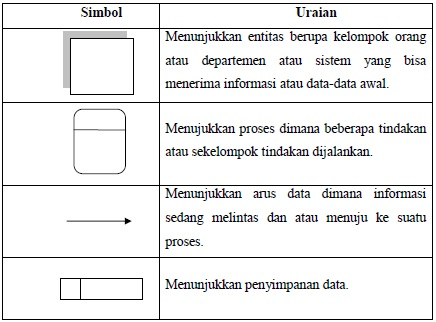
\includegraphics[width=0.6\textwidth]{gambar/1}
    \caption{Entity Relationship Diagram (ERD)}
    \label{wsn}
\end{table}
\newpage

\paragraph{}
Entity Relationship Diagram merupakan diagram yang berisi komponenkomponen himpunan entitas dan himpunan relasi yang masing-masing dilengkapi dengan atribut-atribut yang merepresentasikan seluruh fakta yang ditinjau (Fatansyah, 1999 : 70). Berikut ini merupakan simbol-simbol yang digunakan dalam pembuatan ERD

\begin{table}[ht!]
  \centering
    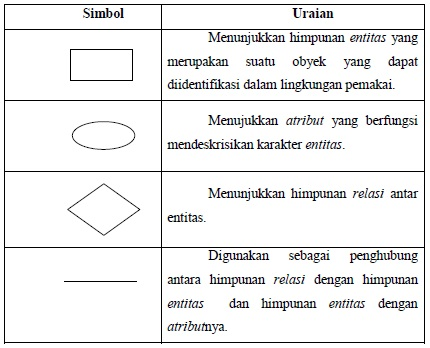
\includegraphics[width=0.6\textwidth]{gambar/2}
    \caption{Tabel Simbol dalam ERD}
    \label{wsn}
\end{table}
\newpage

\section{Perancangan Sistem}
Perancangan sistem merupakan tahap pemasukan ide atau gagasan guna memenuhi suatu tujuan pembangunan sistem informasi sebagai persiapan untuk melakukan rancang bangun dan implementasi. Tahap-tahap dalam perancangan sistem, antara lain adalah dengan pembuatan \textit{Flowchart}, dan \textit{Deskripsi Data} 



\section{Kerelasian Antar Relasi (\textit{Relationship})}
Kerelasian menyatakan hubungan antar relasi dalam basis data. Kerelasian antar relasi dituliskan oleh foreign key atau relasi-relasi bertipe transaksi yang digunakan dalam basis data. Jenis-jenis kerelasian antar relasi, meliputi :
\begin{itemize}
\item[1]Kerelasian satu ke satu (one to one relationship)
\\
Kerelasian satu ke satu terjadi jika setiap nilai pada suatu relasi hanya mengimplikasikan sebuah nilai pada relasi lain yang direlasikan secara logik.
\item[2]Kerelasian satu ke banyak (one to many relationship)
\\
Kerelasian satu ke banyak terjadi jika setiap nilai pada suatu relasi mengimplikasikan banyak nilai pada relasi lain yang direlasikan secara logik.
\item[3]Kerelasian banyak ke satu (many to one relationship)
\\
Kerelasian banyak ke satu terjadi jika banyak nilai pada suatu relasi mengimplikasikan satu nilai pada relasi lain yang direlasikan secara logik.
\item[4]Kerelasian banyak ke banyak (many to many relationship)
\\
Kerelasian banyak ke banyak terjadi jika banyak nilai pada suatu relasi mengimplikasikan banyak nilai pada relasi lain yang direlasikan secara logik.
\end{itemize}


\section{Database (Basis Data)}
Database (basis data) merupakan kumpulan data yang saling berhubungan satu dengan yang lainnya, tersimpan di perangkat keras komputer dan digunakan perangkat lunak untuk memanipulasinya. Untuk membentuk suatu database diperlukan jenjang data, sebagai berikut :
\begin{itemize}
\item[1]Karakter
\\
Karakter merupakan bagian data yang terkecil, dapat berupa karakter numerik, huruf ataupun karakter khusus yang membentuk suatu item data.
\item[2]Field
\\
Field merupakan gambaran suatu atribut dari record yang menunjukkan item dari data.
\item[3]Record
\\
Record merupakan kumpulan dari field-field. Record menggambarkan suatu unit data individu tertentu.
\item[4]File
\\
File terdiri dari dari record-record yang menggambarkan satu kesatuan data yang sejenis.

\item[5]Database
\\
Database merupakan kumpulan dari file.
\end{itemize}



\chapter{DESAIN DAN PERANCANGAN}

Desain dan perancangan memuat tentang data – data yang dibutuhkan dalam pembuatan SMS Gateway sehingga peneliti mengetahui proses – proses yang dibutuhkan dalam pembuatan system.
\section{Perancangan Sistem}
Pembuatan sistem informasi nilai berbasis SMS Gateway Program Diploma Universitas Muhammadiyah Jember dibuat dengan menggunakan java jdk1.6.0 dengan editor EclipseJ2ME dan database MySQL . Dengan menggunakan Software tersebut sistem ini diharapkan dapat membantu kinerja karyawan yang ada di instansi Program Diploma  Universitas Muhammadiyah Jember.

\subsection{Aliran Data}
\begin{itemize}
\item[A]Hierarki

\begin{figure}[ht!]
  \centering
    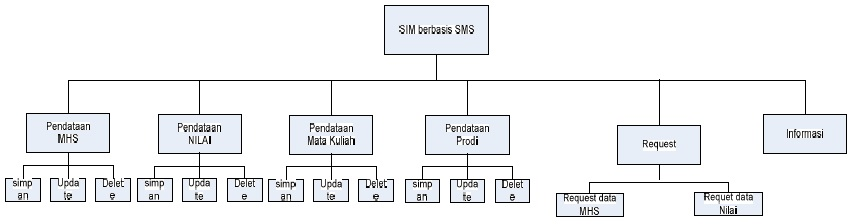
\includegraphics[width=1\textwidth]{gambar/3}
    \caption{Hierarki}
    \label{wsn}
\end{figure}
\newpage

\item[B]\textbf{Data Flow Diagram (DFD)}
\\
Data Flow Diagram merupakan model yang menggambarkan sistem sebagai jaringan kerja antar fungsi yang saling berhubungan dengan aliran dan penyimpanan data.
\begin{itemize}
\item[-] \textbf{DFD Level 0}
\begin{figure}[ht!]
  \centering
    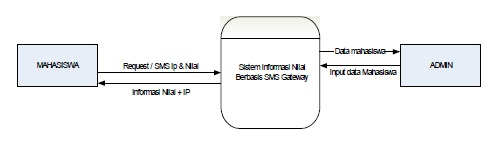
\includegraphics[width=0.7\textwidth]{gambar/4}
    \caption{DFD Level 0}
    \label{wsn}
\end{figure}

\item[-] \textbf{DFD Level 1}
\begin{figure}[ht!]
  \centering
    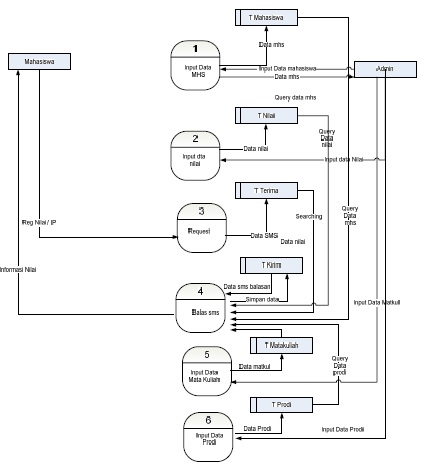
\includegraphics[width=0.7\textwidth]{gambar/5}
    \caption{DFD Level 0}
    \label{wsn}
\end{figure}
\end{itemize}
\end{itemize}

\section{Flowchart}
Flowchart merupakan diagram alur yang menggambarkan urutan logika dari suatu prosedur yang ada dalam suatu sistem.
\begin{figure}[ht!]
  \centering
    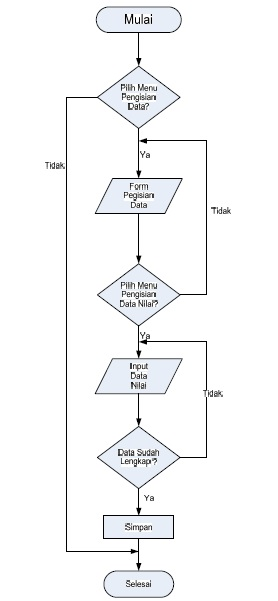
\includegraphics[width=0.5\textwidth]{gambar/6}
    \caption{DFD Level 0}
    \label{wsn}
\end{figure}


\chapter{IMPLEMENTASI DAN EVALUASI}
\section{Implementasi}
Tampilan utama dalam program utama SMS Gateway Program Diploma adalah halaman informasi sms masuk, sms keluar dan link untuk menuju halaman input data mahasiswa. Sedangkan tampilan dalam program pengisian data mahasiswa terdapat dua menu yaitu menu file dan pengisian data, menu file terdapat sub menu keluar yang digunakan untuk keluar dari program. Dan menu pengisian data terdapat dua submenu yaitu submenu pengisian data mahasiswa dan submenu pengisian nilai mahasiswa yang digunakan untuk menginput datamahasiswa.

\subsection{Implementasi antar muka}
\begin{itemize}
\item[a)]Form Mulai
Form mulai merupakan form untuk masuk ke program utama yang berisi informasi pengaturan port dan pengaturan AT Command. AT Command adalah perintah-perintah yang digunakan dalam komunikasi dengan serial port. Dengan AT Command kita dapat mengetahui vendor dari Handphone yang digunakan, kekuatan sinyal, membaca pesan yang ada pada SIM Card, megirim pesan, mendeteksi pesan SMS baru yang masuk secara otomatis, menghapus pesan pada SIM Card dan masih banyak lagi. Form MULAI akan muncul setelah admin mengklik file pasca.bath. Setelah form ini muncul, klik button MULAI kemudian form akan menuju kehalaman utama.
\begin{figure}[ht!]
  \centering
    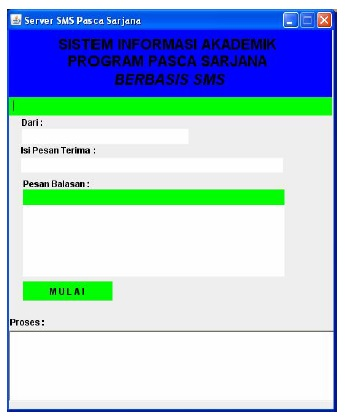
\includegraphics[width=0.5\textwidth]{gambar/7}
    \caption{Form Mulai}
    \label{wsn}
\end{figure}
\newpage

\item[b)]Form Utama
Form utama berisi tampilan waktu, kolom – kolom yang berisi data – data sms yang masuk dan keluar ke pengirim, tombol untuk menutup aplikasi dan tombol untuk masuk ke halaman pengisian database, tombol TUTUP digunakan untuk menutup aplikasi, sedangkan tombol PengisianDatabase Mahasiswa digunakan untuk mengisi data mahasiswa. Dibawah tombol TUTUP terdapat panel proses yang berisi proses – proses yang terjadi saat system membaca ataupun mengirim sms. Proses akan membaca sms yang masuk secara otomatis setiap dua detik dan akan membalas secara otomatis.
\begin{figure}[ht!]
  \centering
    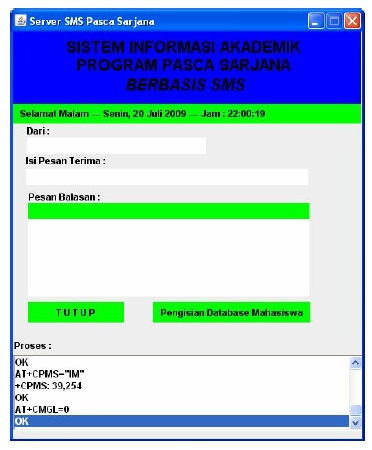
\includegraphics[width=0.5\textwidth]{gambar/8}
    \caption{Form Utama}
    \label{wsn}
\end{figure}
\newpage

\begin{figure}[ht!]
  \centering
    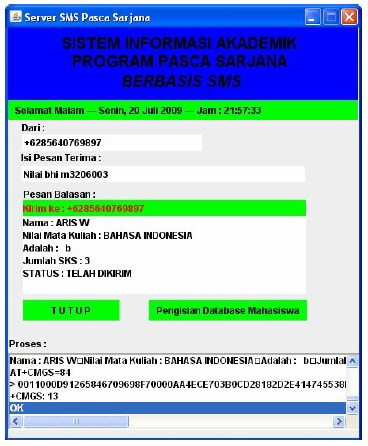
\includegraphics[width=0.5\textwidth]{gambar/9}
    \caption{Contoh Program saat ada sms Masuk}
    \label{wsn}
\end{figure}
\newpage

\item[c)]Form input data Mahasiswa
Form pengisian data merupakan form yang digunakan untuk mengisi data – data mahasiswa. Dalam mengisi data ini semua isian wajib diisi, jika masih terdapat isian yang kosong maka sisteeem tidak dapat menyimpan data. Jika semua isian sudah diisi maka tekan tombol simpan.
\begin{figure}[ht!]
  \centering
    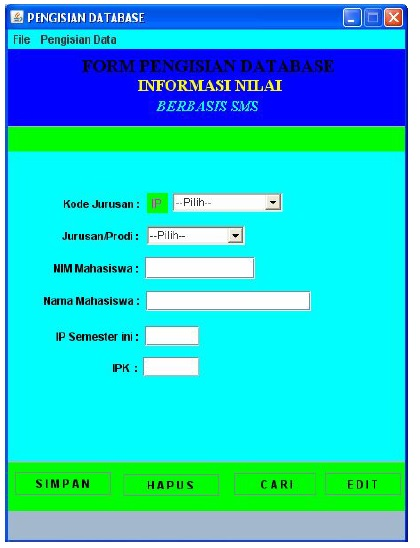
\includegraphics[width=0.5\textwidth]{gambar/10}
    \caption{Form pengisian data mahasiswa}
    \label{wsn}
\end{figure}


\begin{figure}[ht!]
  \centering
    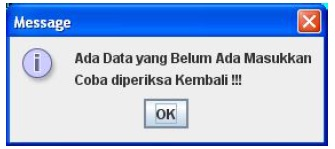
\includegraphics[width=0.5\textwidth]{gambar/11}
    \caption{Pesan peringatan input data belum lengkap}
    \label{wsn}
\end{figure}
\newpage

\begin{figure}[ht!]
  \centering
    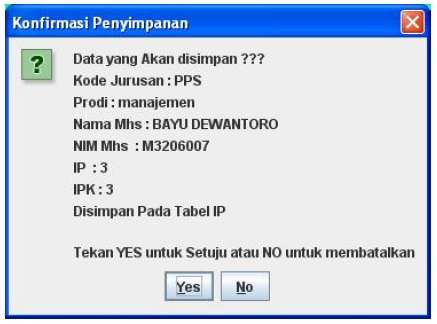
\includegraphics[width=0.5\textwidth]{gambar/12}
    \caption{Contoh konfirmasi penyimpanan}
    \label{wsn}
\end{figure}

\begin{figure}[ht!]
  \centering
    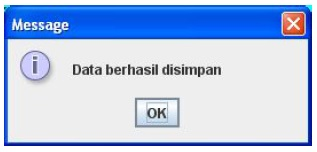
\includegraphics[width=0.5\textwidth]{gambar/13}
    \caption{Laporan saat data berhasil disimpan}
    \label{wsn}
\end{figure}

\item[d)]Form Input Nilai mahasiswa
Form input nilai mahasiswa merupakan form yang digunakan untuk mengisi nilai – nilai mahasiswa.saat menginput data ini semua isian wajib diisi.
\begin{figure}[ht!]
  \centering
    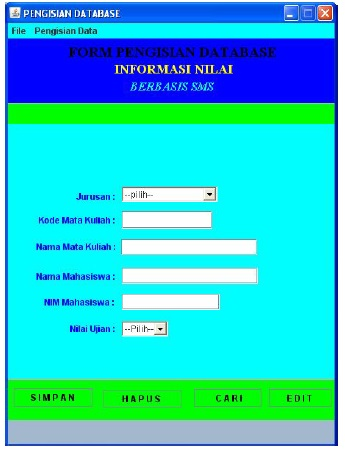
\includegraphics[width=0.5\textwidth]{gambar/14}
    \caption{Form Input data nilai}
    \label{wsn}
\end{figure}
\newpage

\item[e)]Tombol edit
Saat tombol edit ditekan maka akan muncul kotak dialog permintaan untuk mengisi NIM

\begin{figure}[ht!]
  \centering
    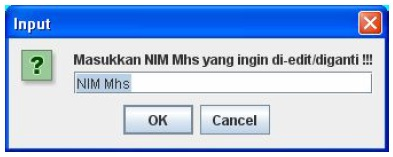
\includegraphics[width=0.5\textwidth]{gambar/15}
    \caption{Form Edit}
    \label{wsn}
\end{figure}

\end{itemize}

\section{Evaluasi Sistem}
Sistem informasi nilai berbasis SMS Gateway merupakan suatu sistem informasi yang menangani informasi – informasi nilai kepada mahasiswa sehingga mahasiswa dapat mengakses darimanapun mahasiswa tersebut berada. Informasi disini meliputi informasi nilai IPK, IP semester dan informasi nilai ujian mahasiswa.
Kelemahan dari sistem ini yaitu lamanya proses membalas sms, hal ini terjadi karena pada saat mencari data, system harus membaca setiap proses yang ada dalam system.
\paragraph{}
Kelebihan dari sistem ini yaitu cara mengoperasikan yang begitu mudah sehingga dapat digunakan oleh admin manapun. Sistem ini dapat mengatasi masalah yang berkaitan dengan pemberian informasi – informasi nilai kepada mahasiswa yang selama ini masih dilakukan secara offline artinya mahasiswa tidak dapat mengakses nilai mereka dari mana saja sehingga dengan adanya sistem ini diharapkan dapat membuat pekerjaan karyawan program Diloma  Universitas Muhammadiyah Jember  lebih efisien .

\chapter{PENUTUP}
\section{Kesimpulan}
Dari hasil penelitian penulis mengambil kesimpulan sebagai berikut :
\begin{itemize}
\item[1]Sistem informasi nilai berbasis SMS Gateway merupakan suatu sistem yang menangani informasi – informasi nilai kepada mahasiswa secara on line
\item[2]Dibangunnya sistem ini dapat mempercepat informasi nilai dan ip yang dibutuhkan tanpa harus menunggu versi tercetak yang relatif lebih lama.
\end{itemize}

\section{Saran}
Dari hasil penelitian, penulis memberikan saran agar pada tahap selanjutnya dilakukan pengembangan dan perbaikan sistem terutama pada proses balas sms yang lama karena harus melalui beberapa proses.

\begin{thebibliography}{9}

\bibitem[satu(2015)]{satu01}
Ariyanto, 2005, \textit{Pengembangan Aplikasi Sistem Informasi Akademik Berbasis SMS dengan JAVA}, Jakarta, Salemba Infotek

\bibitem[tiga(2015)]{tiga03}
Fathansyah, 1995, Basis Data Informatika, Bandung

\bibitem[empat(2015)]{empat04}
Kendall. 2003. Analisis dan Perancangan Sistem. PT Intan Sejati : Klaten

\bibitem[lima(2015)]{lima05}
Kristanto. H, 1993, Konsep dan Perancangan Database, Jogjakarta, Andi offset

\bibitem[enam(2015)]{enam06}
Susanto. M. J, 1995, Manajemen Database dengan Sql, Jakarta, Dinastindo

\bibitem[tujuh(2015)]{tujuh07}
Sutedjo, B. dan Michael AN. 2000. Algoritma dan Teknik Pemrograman Konsep,Implementasi, dan Aplikasi. Andi : Yogyakarta

\end{thebibliography}
\addcontentsline{toc}{chapter}{DAFTAR PUSTAKA}
%-----------------------------------------------------------------
%Disini akhir masukan Daftar Pustaka
%-----------------------------------------------------------------

\end{document}